\documentclass[../main.tex]{subfiles}
\graphicspath{
		{"../img/"}
		{"img/"}
}

\begin{document}
		Mamy za sobą metodę charakterystyk, zobaczyliśmy, że przedstawienie problemu jako równania całkowego pozwala na poszerzenie dziedziny rozwiązań. Dobrzy byłoby wrócić do równania Hamiltona-Jacobiego i zobaczyć w nim charakterystyki, na razie jednak zajmiemy się metodą separacji zmiennych
		\subsection{Metoda separacji zmiennych}
		\begin{przyklad}
				Niech $u: (x,y)\subset\mathbb{R}^2\to \mathbb{R}$, taka, że
				\[
						u_{,x} + 2u_{,y} = 3
				.\]
		\end{przyklad}
		Moglibyśmy rozwiązać to równanie charakterystykami, ale spróbujemy inaczej. Załóżmy, że
		\[
				u(x,y) = p(x) + q(y),\quad p,q:\mathbb{R}\to \mathbb{R}
		.\]
		Dlaczego akurat tak? Gdybyśmy mieli twierdzenie o jednoznaczności, to nie musielibyśmy przejmować się dzielnymi założeniami - skoro działa to znaczy, że jest ok.\\
		Po podstawieniu otrzymujemy
		\[
				p'(x) + 2q'(y) = 3
		,\]
		czyli
		\[
				p'(x) = 3-2q'(y) \underset{x,y\in X\subset\mathbb{R}^2}{\forall}
		.\]
		Oznacza to, że prawa i lewa strona powinny mieć tą samą wartość niezależnie od $x$ i $y$. Czyli
		\begin{align*}
				\underset{k}{\exists}\quad p'(x) &= k \implies p(x) = kx + c_1\\
						3-2q'(y) &= k \implies q(y) = \frac{3-k}{2} y + c_2
		.\end{align*}
		Zatem
		\[
				u(x,y)_k = kx + c_1 + \frac{3-k}{2} y + c_2
		.\]
		To ile to $k$ powinno wynosić? Problem jest addytywny, więc moglibyśmy zsumować lub scałkować wszystkie $u(x,y)_k$.
		\[
				\left[ u_{,t}+u_{,x} \right] \begin{bmatrix} a\\b \end{bmatrix} = 0 \implies \nabla_{[a,b]}u = 0
		.\]
		Czyli $u$ - stała na poziomicy i $u(x,t) = f(bt-ax)$.\\
		Widzimy, że poprzednie rozwiązanie nie było najogólniejsze na świecie. To po co nam superpozycja? \textbf{Bo szybko wychodzi.}
		 \begin{przyklad}
				 niech dla $u(x,0) = g(x)$,
				 \[
				 u_{,t} + au_{,x} = 0
				 .\]
				 Wiemy, że $u = g(x-at)$.\\
				 Zamiast tego załóżmy, że
				  \[
						  u(x,t) = X(x) \cdot T(t)
				 ,\]
				 czyli
				 \[
						 X(x) \cdot T_{,t}(t) + aT(t) \cdot X_{,x}(x) = 0
				 .\]
				 Dalej
				 \[
						 \frac{T_{,t}(t)}{T(t)} = -a \frac{X_{x}(x)}{X(x)} \underset{X,T \neq 0}{\forall}
				 .\]
				 Czyli w tej konwencji

				 \[
						 \frac{T_{,t}}{T} = -a k,\quad \frac{X_{,x}}{X} = k
				 .\]
				 Czyli
				 \[
						 X(x) = B_k e^{kx},\quad T(t) = A_ke^{-kat}
				 ,\]
				 zatem
				 \[
						 u(x,t,k) = c_k e^{k\left( x-at \right) }
				 .\]
				 Pisząc z sumami wyjdzie tak
				 \[
						 u(x,t) = \sum c(k) e^{k(x-at)},\quad u(x,0) = \sum A_k e^{kx} = g(x)
				 .\]
				 A bez sum, to tak samo, tylko bez sum.
		\end{przyklad}
				 Widzimy, że powyższe podejście wyznacza klasę $g$ funkcji, która mogłaby zadać warunek brzegowy oraz klasę funkcji, na które chcemy rozwinąć warunek brzegowy. Językiem, który pozwoli opisać problem będzie język algebry. Popatrzmy na równania:
				 \begin{align}
						 \label{eq:separ}
						 X_{,x}(t) &= k X(x)\\
						 T_{,t}(t) &= -ak T(t)
				 \end{align}
				 w sposób następujący. Niech $L_1 = \frac{\partial }{\partial x}$, $X(x) = \psi_1$, $\frac{\partial }{\partial t} = L_2$, $T(t) = \psi_2$, $ak = \lambda_2$. Wtedy \ref{eq:separ} wygląda bardziej jak na kwantach
				 \[
				 L_1\psi_1 = k\psi_1,\quad L_2\psi_2 = \lambda_2\psi_2
				 .\]
				 Na algebrze pojawiały się podobne napisy, tylko że wyglądały tak $A v = \lambda v$.
				 Wychodzi na to, że jak się postaramy, to będziemy mogli związać z np. operatorem $\partial_x$ jego wektory własne!\\
				 W naszym przypadku by to miało postać
				 \[
						 \psi_1(x) = e^{xk},\quad \psi_2(t) = e^{-\lambda t}
				 .\]
				 Jeżeli dołożymy do tego liniową niezależność, to będziemy mogli pytać o bazę rozwiązań, o to, jakie warunki brzegowe da się w takiej bazie przedstawić i jak zszyć ze sobą wartości własne $\lambda_1$ i $\lambda_2$ ($k$ i $-ak$ ). Wartości własne muszą być funkcjami sensownej klasy (sensowna = fajna).
				 Pamiętamy, że z $L^1$ nie zwiążemy iloczynu skalarnego z normą supremum (a ona jest przecież najfajniejsza na świecie).
				 W większej niż jeden liczbie wymiarów dochodzi jeszcze problem dziedziny wartości własnych.
				 Nikt nam nie przeszkodzi w znajdowaniu funkcji własnych dla membrany okrągłęj (bębna), ale dla membran ładnych inaczej \ref{fig:ladneinaczej} już jak najbardziej. Nawet nie chodzi nam tutaj o trudności w rachunkach, tylko bardziej o istnienie rozwiązań).
				 \begin{figure}[h]
				 		\centering
				 		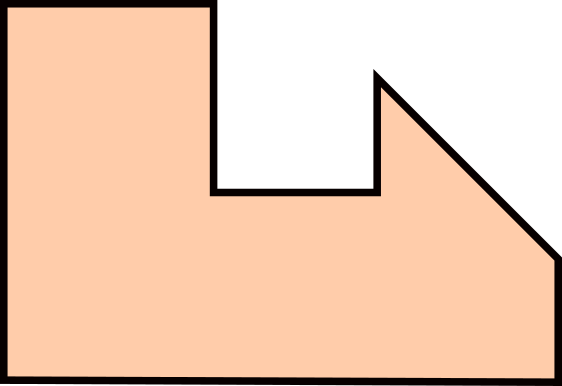
\includegraphics[width=0.4\textwidth]{ladneinaczej}
				 		\caption{Membrana ładna inaczej, czyli w zasadzie dowolna niepodobna do elipsy}
				 		\label{fig:ladneinaczej}
				 \end{figure}

				 Inną przydatą rzeczą, jest umiejętność rozwiązania problemu odwrotnego - mając rozwiązanie znaleźć warunek początkowy. Na przykład mając sygnał z tomografu chcemy odtworzyć to w co on strzelał.\\
				 Widzimy zatem, że metoda separacji bynajmniej nie jest konstrukcją naturalną i na wiele rzeczy nam nie pozwoli (nawet na takie niewinne rzeczy jak potencjał zmienny w czasie).\\
				 A na co pozwala?
				 \begin{przyklad}
				 		Rozważmy równanie $u_t = u_{x x}$ dla $0<x<\pi$ i $t > 0.$
						Jeszcze nałożymy warunek brzegowy
						 \[
								 u(0,t) = u(\pi,t) = 0
						 ,\]
						 czyli na początku i na końcu mocowania ma się zerować.\\
						 Zastosujemy separację zmiennych:
						 \[
								 u(x,t) = y(x) g(t) \implies y(x)g'(t) = g(t)y''(x)
						 .\]
						 Warunek brzegowy zmnienia się w taki ładny układ
						 \begin{align*}
								 y(0)g(t) &= 0\\
								 y(\pi)g(t) &= 0
						 .\end{align*}
						 Zatem
						 \[
								 \frac{y''(x)}{y(x)} = \frac{g'(t)}{g(t)} = -\lambda
						 .\]
						 Czyli
						 \[
								 g'(t) = -\lambda g(t),\quad y''(x) = -\lambda y(x)
						 .\]
						 No to trzeba rozwiązać, wyjdzie
						 \[
								 g(t) = A_\alpha e^{-\lambda t},\quad
								 \begin{cases}
										 y''(x) + \lambda y(x) = 0& 0 <x<\pi\\ y(0) = y(\pi) = 0
								 \end{cases}
						 .\]
						 Co to znaczy $\lambda$? To jest ujemne, czy dodatnie?\\
						 Gdyby $\lambda = -\alpha^2$, to wtedy
						 \[
								 y(x) = Ce^{\alpha x} + D e^{-\alpha x}
						 ,\]
						 co nie mogłoby spełnić warunku brzegowego. To może inaczej.\\
						 Niech $\lambda = \alpha^2$, wtedy
						 \[
								 y(x) = A_\alpha \cos(\alpha x) + B_\alpha \sin(\alpha x)
						 .\]
						 Pierwszy wyraz nam odpada, bo $y(0) = 0$, a z drugiego warunku wynika
						 \[
								 y(\pi) = 0 \implies B_\alpha \sin(\alpha\pi) = 0
						 .\]
						 Czyli $\alpha = n \implies \lambda = n^2$. To fajnie nawet się ułożyło, można podstawić do $u(x,t)$,
						 \[
								 u_n(x,t) = A_n e^{-n^2 t} \sin(nx)
						 .\]
						 A jak się przesumuje po $n$, to będzie tak samo tylko z sumą po $n$.
						 Pamiętamy, że
						 \[
								 u(x,0) = \sum_n A_n \sin(nx)
						 .\]
						 Czyli mamy fouriera. Współczynniki liczymy jak zawsze,
						 \[
								 A_n = \frac{2}{\pi}\int\limits_{0}^\pi d\xi \sin\left( n\xi \right) u(\xi, 0)
						 .\]
						 Można podstawić do wzoru na $u(x,t)$
						 \begin{align*}
								 u(x,t) &= \frac{2}{\pi}\sum_n \int\limits_0^\pi \sin(n\xi)u(\xi,0)d\xi \cdot \sin(n x) e^{-n^2 t} = \\
								 &= \frac{2}{\pi}\int\limits_0^\pi d\xi \left( \sum_n \sin(n\xi) \sin(nx) e^{-n^2 t} \right) u(\xi,0)
						 .\end{align*}
				 \end{przyklad}
				 Co z jednoznacznością, rodzajem zbieżności i tak dalej?\\
				 Ograniczmy się tutaj do takich operatorów, które pojawiają się w równaniach fizyki matematycznej przy okazji separacji zmiennych w postaci iloczynu (wtedy można mówić o wartościach własnych).
				 \subsection{Operatory Sturma-Liouville'a}
		Niech $p,q,r \in \mathcal{C}^2[a,b]$ spełniające $p(x) > 0$, $q(x) > 0$, $a \le x \le b$. Będziemy szukać rozwiązań problemu
		\[
				-\frac{d}{dx}\left( p(x) \frac{dv}{dx} \right) + q(x)v(x) = \lambda r(x) v(x)
		.\]
		$\lambda\in \mathbb{C}$.\\
		Iloczyn skalarny dany tak
		\[
				\left<u|v \right> = \int\limits_a^b \overline{v(x)} u(x) r(x) dx
		.\]
		Więc norma to
		\[
		\Vert f \Vert = \left<f|f \right>^{\frac{1}{2}}
		.\]
		Nie jest zbyt wygodna dla szacowań, wolelibyśmy $sup$, ale nie dostaniemy takiej z iloczynu skalarnego.
		\begin{przyklad}
				Równanie Schr\"odingera po separacji zmiennych
				\[
						-\frac{\hbar^2}{2m}\psi'' + V(x)\psi = E\psi
				.\]
				Czyli operator jest postaci
				\[
						L(v) = -\frac{1}{r(x)}\left[ \frac{d}{dx}\left( p(x)\frac{dv}{dx} \right) + q(x)v \right]
				,\]
				gdzie $\frac{p}{r} = \frac{\hbar^2}{2m}$, $\frac{q}{r} = E-V$.
				Dla niego wektor własny spełnia $L(v) = \lambda v$. \\
				Przykładowe warunki brzegowe
				\begin{itemize}
						\item pudełko - $\psi(0) = 0$, $\psi(L) = 0$
						\item okrąg -  $\psi(0) = \psi(L)$
				\end{itemize}
		\end{przyklad}
		Do czego potrzebny nam iloczyn skalarny? Pamiętamy z algebry, że na przestrzeni Hilberta wektory własne, (jeżeli operator jest wystarczająco fajny) są prostopadłe w danym iloczynie skalarnym. Aby tak było, $L$ musi spełniać warunek
		\[
		\left<L f|g \right> = \left<f|Lg \right>
		.\]
		To oznacza, że
		\begin{align*}
				\left<Lf|g \right> &= \int\limits_a^b (Lf)(x)\overline{g(x)} r(x)dx = \int_a^b\left( -(p(x)f')' + q(x)f \right) \overline{g(x)} = \\
				&= - \int\limits_a^b \left( (p(x)f')'\overline{g(x)} + q(x)f(x)\overline{g(x)}  \right) dx = \\
				&= -\left.p(x)f'(x) \overline{g(x)} \right|_a^b - \int\limits_a^b\left( -p(x)f'(x)\overline{g'(x)} + q(x)f(x)\overline{g(x)}  \right) dx
		.\end{align*}
		Prawa strona
		\begin{align*}
				\left<f|Lg \right> &= \int\limits_a^bf(x)\overline{\left( -p(x)g'(x) \right) '}  - q(x)f(x)\overline{g(x)} = \\
				&= -\left.p(x)\overline{g'(x)}f(x)\right|_a^b - \int\limits_a^b\left( -p(x)\overline{g'(x)} f'(x) + q(x)f(x)\overline{g(x)}  \right) dx
		.\end{align*}
		Czyli lewa strona minus prawa strona
		\[
				\left<f|Lg \right> - \left<Lf|g \right> = \left.p(x)f'\overline{g(x)} - p(x)\overline{g'(x)} f(x)\right|_a^b
		.\]
		Jeżeli
		\begin{itemize}
				\item $p(a) = p(b) = 0$, to $\left<Lf|g \right> = \left<f|Lg \right>$.
				\item $f,g\in \mathcal{L}^2$, $[a,b]\to]-\infty,\infty[$ to też może być ok,
				\item możliwe oczywiście też inne warunki.
		\end{itemize}
		Przypomnienie z algebry - jeżeli $\left<Lf|g \right> = \left<f|Lg \right>$, to mówimy, że operator jest samosprzężony, wówczas
		\begin{itemize}
				\item wszystkie jego wartości własne są rzeczywiste
						\begin{align*}
								\lambda\Vert u \Vert ^2 &= \lambda \left<u|u \right> = \left<\lambda u|u \right> = \left<L u|u \right> =\\
						&= \left<u|Lu \right> = \left<u|\lambda u \right> = \overline{\lambda} \left<u|u \right> = \overline{\lambda} \Vert u \Vert ^2
						.\end{align*}
				\item wektory własne odpowiadające różnym wartościom własnym są prostopadłe
		\end{itemize}
		To znaczy, że jeżeli $u$, $v$ są takie, że
		\[
		Lu = \lambda u,\quad Lv = \lambda v
		,\]
		to
		\[
		v L u - u L v = v \lambda u - u \lambda v = 0
		.\]
		No i co z tego? ano
		\[
				-v \frac{d}{dx}\left( p(x)u' \right) + u \frac{d}{dx}\left( p(x) v' \right) = 0
		,\]
		czyli
		\[
				\frac{d}{dx}\left( p(x)(uv' - u'v) \right) = 0
		.\]
		Zatem
		\[
				p(x) \left( u(x)v'(x) - u'(x)v(x) \right) = const \underset{x\in[a,b]}{\forall}
		.\]
		Jak połączymy to z warunkiem brzegowym, to dostaniemy
		\[
				p(x) \left. \left( \overline{u(x)} v'(x) - \overline{u'(x)} v(x) \right) \right|_a^b = 0
		.\]
		Co by było jakby $\overline{u(a)} v'(a) - \overline{u'(a)} v(a) = 0$?\\
		No wtedy to jest fajnie, bo $\underset{x}{\forall} u(x)v'(x) - u'(x)v(x) = 0$, czyli
		\[
				\det\begin{bmatrix} u(x)&v(x)\\u'(x)&v'(x) \end{bmatrix} = 0
		.\]
		A to oznacza, że kolumny są liniowo zależne. Czyli jeżeli
		 \[
		Lu = \lambda u,\quad Lv = \lambda v \implies \underset{c}{\exists} u = cv
		.\]
		A co jeżeli
		\begin{align*}
				p(a)\left[\overline{u(a)}v'(a) - \overline{u'(a)}v(a)\right] &= const \neq 0\\
				p(b)\left[\overline{u(b)}v'(b) - \overline{u'(b)}v(b)\right] &= const \neq 0\\
		?\end{align*}
		Warunek na samosprzężoność jest spełniony, ale
		\[
				\det\begin{bmatrix} u&v\\v'&v' \end{bmatrix} \neq 0
		,\]

		czyli dla tej samej $\lambda$ mamy dwa różne rozwiązania. Znajomość $\lambda$ i samosprzężoność nie dają jednoznaczności rozwiązań. W ten sposób różnią się rozwiązania o periodycznych warunkach brzegowych (np na okręgu) od struny zamocowanej na obu końcach.
		\begin{przyklad}
				\[
				-y'' = \lambda y,\quad -\pi\le y\le \pi
				.\]
				warunki periodyczne $y(-\pi) = y(\pi)$, $y'(-\pi) = y'(\pi)$.
				Wartości własne to $\mathbb{N}\ni n^2$, a wektory własne to
				\begin{align*}
						u_n^1&= \cos(nx)\\
						u_n^2&= \sin(nx)
				.\end{align*}
				Osobną sprawą jest znak wartości własnych i to, czy są one ograniczone np. od dołu, żeby przypominało na przykład energię.
		\end{przyklad}
\end{document}
